\documentclass[11pt]{article}
\usepackage[margin=0.75in]{geometry}
\usepackage[T1]{fontenc}
\usepackage[scaled]{helvet}
\renewcommand{\familydefault}{\sfdefault}
\usepackage{xcolor}
\usepackage{titlesec}
\usepackage{enumitem}
\usepackage{graphicx}
\usepackage[font=small,labelfont=bf,skip=6pt]{caption}
\usepackage[hidelinks]{hyperref}

\titleformat{\section}{\normalsize\bfseries}{}{0pt}{}
\titlespacing*{\section}{0pt}{8pt}{3pt}
\setlength{\parindent}{0pt}
\setlength{\parskip}{5pt}
\pagestyle{empty}

% Placeholders still to be filled
\newcommand{\tbc}[1]{\textcolor{red}{[#1]}}

\begin{document}

{\large\bfseries Specific Aims: Phenotypic Plasticity in Cancer Metastasis}\\[2pt]
{\small Kishore Hari \,\textperiodcentered\, Draft for discussion, November 11, 2026}

Metastasis causes most cancer deaths, yet the cell states that let a cancer cell leave the primary tumour, survive in circulation and colonize a distant organ remain poorly defined. A recurring feature of this process is phenotypic plasticity: cells move along the epithelial--mesenchymal (E--M) axis and can occupy hybrid E/M states that combine migratory traits with adhesion and stemness. Hybrid E/M cells have been associated with higher metastatic potential, but we lack a quantitative account of which kinds of plasticity matter, and at which stage of metastasis.

Two gaps limit progress. Metastasis is observed in snapshots, so the order and timing of state changes are rarely known. And models of EMT dynamics are seldom confronted with data from metastatic settings, or with the microenvironment that shapes plasticity, such as cancer-associated fibroblasts (CAFs) and immune cells.

We propose to treat a cell's position on the E--M axis as an order parameter that links gene regulatory network (GRN) dynamics to tumour-scale behaviour. \textbf{Central hypothesis:} metastatic success depends on a specific form of plasticity, in which hybrid states are stable enough to persist yet reversible enough to switch in response to microenvironmental signals. Our multilevel Boolean models suggest that graded regulation can stabilize otherwise fragile hybrid states, which gives this hypothesis a mechanistic starting point.

\begin{figure}[t]
  \centering
  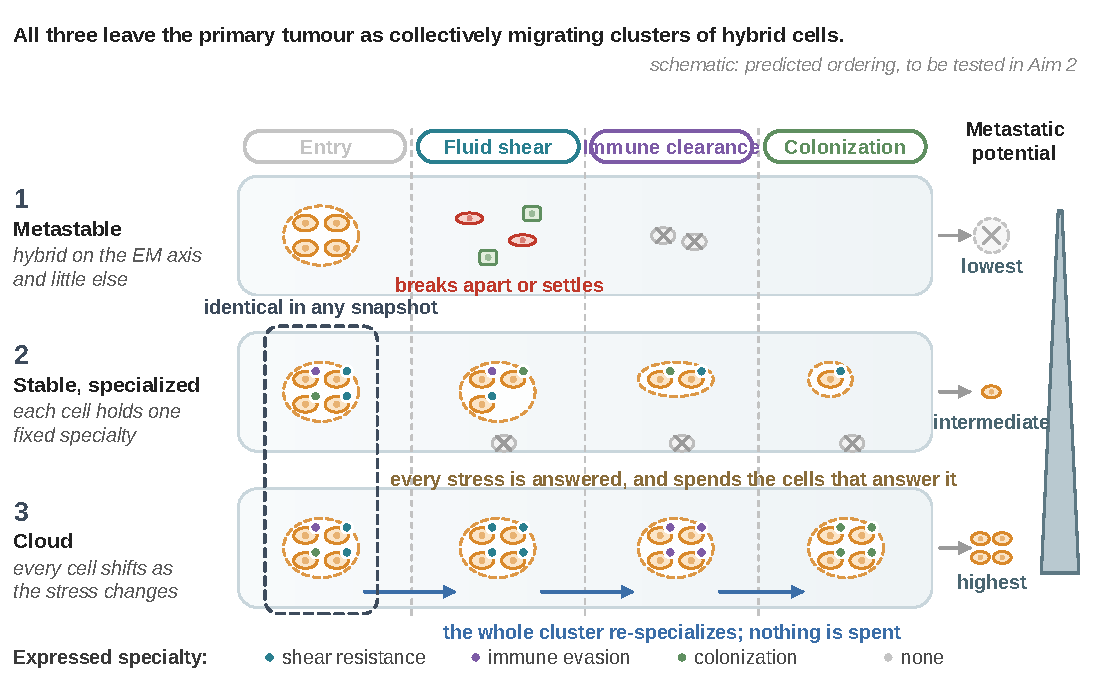
\includegraphics[width=\textwidth]{Fig1.pdf}
  \caption{Metastatic cells can show different kinds of phenotypic dynamics, each trading off
  robustness against plasticity. We aim to identify which dynamics occur at, and are suited to,
  each stage of metastasis, through multi-omics integrated mathematical modelling. Axis positions
  are conceptual; the project would place each regime quantitatively, by switching rate against
  residence time in a state.}
  \label{fig:regimes}
\end{figure}

\section{Aim 1. Build a time-resolved map of EMT-state heterogeneity across metastasis}

We will assemble public datasets that pair transcriptomic, DNA methylation and genomic profiling across primary tumours, circulating tumour cells and metastatic sites, such as the AURORA US and BIG cohorts of matched primary--metastasis pairs, and score each sample on the E--M axis. Genomic profiles let us ask whether a shifted EMT state accompanies a clonal change or arises without one, which separates plasticity from selection of a genetic variant. To place samples in time, we will estimate each tumour sample's mitotic age with a fluctuating-CpG (fCpG) methylation clock, which resets at the start of tumour growth and has been used to time metastasis in paired primary and metastatic samples. Relating EMT scores to mitotic age and clonal structure would turn snapshots into a timeline of state changes. Chromatin accessibility would speak more directly to whether a hybrid state is epigenetically poised or locked; paired accessibility data from metastatic samples remain scarce, so we would add this layer in Aim 3, where organoids make it feasible.

Integrating these heterogeneous datasets with quantitative findings scattered across the literature is itself a central challenge, and a new direction for me. We will build an agentic AI framework that retrieves and curates datasets, extracts measurements together with their experimental context from papers, and encodes those findings as virtual experiments that each model must reproduce, following the model-specification and virtual-experiment approach of the Ravasz Regan group's \href{https://github.com/Ravasz-Regan-Group/dynmod}{dynmod} framework. The framework would carry this context into Aims 2 and 3, so that each model is constrained by the full body of relevant evidence. \textit{Benchmark:} stage-wise E--M distributions and mitotic-age orderings that are consistent across independent cohorts.

\section{Aim 2. Identify the forms of plasticity that best explain metastatic state distributions}

Using GRN models of EMT (RACIPE ensembles and multilevel Boolean networks), we will generate alternative plasticity regimes: stable hybrid states, rapid switching between E and M, and largely irreversible transitions. Each regime predicts different state distributions and transition patterns across stages. We will couple these models to microenvironmental inputs, namely CAF-derived signals (including the temporal dynamics of fibrotic rings) and immune recruitment, building on our model of T cell infiltration. Each regime will then be compared with the Aim 1 data. \textit{Benchmark:} one regime reproduces the observed stage-wise distributions where the competing regimes fail.

\section{Aim 3. Test model predictions experimentally with the Mani lab}

Building on our ongoing collaboration on hybrid-state plasticity, we will use the best-supported regime from Aim 2 to predict how hybrid-state frequencies and switching respond to perturbation, such as altered EMT-inducing signals or CAF-conditioned environments. The Mani lab would test these predictions in its established organoid models and in tail-vein injection assays of metastatic colonization. Agreement would support the framework; disagreement would show which model assumptions need revision.

\section{Expected outcomes and impact}

The central outcome would be a functional classification of hybrid-state heterogeneity: not a catalogue of intermediate states, but a grouping of them by what they do during metastasis. Such a classification would let us ask which hybrid states survive transit through the bloodstream, and whether any of them can be driven into a non-metastatic fate, the premise behind transdifferentiation therapies. It would also let us explain stage-dependent phenomena, such as why fibrotic rings appear to restrain cells at one stage and aid escape at another, as consequences of the EMT states present at each stage. Beyond these questions, the work would leave behind a validated, reusable modelling framework that could later be extended toward a multiscale model of metastasis. Keeping the models simple and interpretable, as Herbie's group emphasizes, should keep the predictions testable. For my own training, the project adds epigenetic timing of tumour evolution, agentic AI for large-scale context integration, and direct experimental collaboration to my background in network modelling.

\section{Questions for Herbie}
\begin{itemize}[leftmargin=*,itemsep=1pt,topsep=2pt]
  \item Is the central hypothesis sharp enough, or should it name a specific mechanism for stable-yet-reversible hybrid states?
  \item Should both CAF signals and immune recruitment stay in Aim 2, or is one enough for a fellowship-scale project?
  \item Does the agentic AI pipeline read as a credible new skill, or does it distract from the science?
  \item Two-year or three-year plan?
\end{itemize}

\end{document}